\documentclass[a4paper]{article}
\usepackage[parfill]{parskip}
\usepackage{fullpage}
\usepackage{enumitem}
\usepackage[margin=0.9in]{geometry}
\usepackage{hyperref}
\usepackage{blindtext}
\usepackage{multicol}
\usepackage{siunitx}
\usepackage{graphicx}
\usepackage{wrapfig}
\usepackage{capt-of}
\usepackage{multirow}
\newenvironment{colfigure}
  {\par\medskip\noindent\minipage{\linewidth}}
  {\endminipage\par\medskip}

\makeatletter
  \newenvironment{tablehere}
    {\def\@captype{table}}
    {}
  
  \newenvironment{figurehere}
    {\def\@captype{figure}}
    {}
\makeatother

\bibliographystyle{plain}
\begin{document}

\centerline{\large NLP Assignment 2}
\vspace{0.2in}
\centerline{\Large\bf SVM-based Sentiment Detection of Reviews}
\vspace{0.1in}
\centerline{\large {Anik Roy, Christ's (ar899)}}
\vspace{0.1in}
\centerline{\large {\today}}
\vspace{0.05in}
\centerline{Word Count: 995\footnote{Using texcount}}
\vspace{0.2in}


\begin{multicols}{2}
  
\section{Introduction}

Support vector machines (SVMs) are an ML model which can be used to classify vectors. This method can be applied to the task of classifying documents by representing each document as a vector. In this report, I use a neural model, doc2vec, introduced by Mikolov and Le \cite{DBLP:journals/corr/LeM14}, in order to generate feature vectors. I also qualitatively show that the vector space produced by the doc2vec model is meaningful, by examining the behaviour of document embedding generation by doc2vec.

\section{Background}

In a previous report, I represented documents using a bag of n-grams (BOW) representation, and used an SVM to classify these feature vectors. In BOW, each document is represented by a feature-count vector $(n_1(d), \dots ,n_m(d))$, with $n_i(d)$ being the number of occurrences of $f_i$ in $d$. I also used a representation only using the presence of n-grams, setting $n_i(d)$ to 1 if $f_i$ appeared in $d$, and 0 otherwise.

\subsection{SVM}

SVMs are supervised learning models which are used to classify feature vectors in an n-dimensional space. Training consists of finding a hyperplane which separates the two classes with the largest margin. Classification takes place by measuring the distance of feature vectors to the plane. 

\subsection{Doc2Vec}

Doc2Vec is an unsupervised model for learning document embeddings which can be used as feature representations. It tries to overcome two flaws in BOW - word order not being taken into account, and the semantics of words being ignored. Doc2Vec produces fixed-length vectors for documents of arbitrary length. These vectors can't be directly interpreted. \cite{DBLP:journals/corr/LeM14}

Doc2Vec extends word2vec \cite{DBLP:journals/corr/MikolovSCCD13} , a method of learning word embeddings. There are two doc2vec architectures, distributed bag of words (DBOW) and distributed memory (dm).

\section{Method}

I implemented an SVM classifier which used doc2vec representations\footnote{Available at both \url{https://github.com/anik545/Part2-NLP} and at /home/ar899/Part2-NLP on MCS machines}. I used the doc2vec implementation found in gensim \cite{gensim} and the SVMlight \footnote{http://svmlight.joachims.org/} SVM implementation. I used the Stanford Large Movie Review Dataset \cite{maas-EtAl:2011:ACL-HLT2011} in order to train the doc2vec model. This contains 50,000 labelled (positive and negative, balanced) reviews and 50,000 unlabelled. I performed tokenization on this corpus using the nltk package \footnote{https://www.nltk.org/api/nltk.tokenize.html} \cite{bird-loper-2004-nltk}. I also used a smaller labelled and balanced dataset of 2000 tokenised reviews, a modificaion of the reviews used by Pang et al. \cite{pang2002thumbs}, given to us in the framework of an NLP course.

I used the smaller dataset to train the SVM classifier, performing a 10-fold round-robin stratified cross-validation. 

To tune parameters for the doc2vec model, I used a 10\% validation set to evaluate different doc2vec hyperparameters. I employed a naïve search strategy, starting from the parameters used by Lau and Baldwin \cite{lau2016empirical}. After finding the hyperparameters which gave the highest accuracy on the validation set, I discarded all other models.

I compare the doc2vec based SVM model to two baseline svm models using a BOW representation.

\section{Results}

\begin{table*}
  \centering
  \begin{tabular}{llllllll}
  Method & Vector Size & Window Size & Min Count & Epochs & Hierachical Softmax &  &  \\ \cline{1-6}
  DBOW   & 120         & 7           & 15        & 5      & True                &  & 
  \end{tabular}
  \caption{Values for the optimal hyperparameters found for the doc2vec model}
  \label{tab:param-tab}
\end{table*}

\begin{table*}
  \centering
  \begin{tabular}{lllll}
                                            &                                  & \multicolumn{3}{c}{(2)}                                                                            \\ \cline{3-5} 
                                            & \multicolumn{1}{l|}{}            & \multicolumn{1}{l|}{BOW - freq.} & \multicolumn{1}{l|}{BOW - pres.} & \multicolumn{1}{l|}{Doc2vec} \\ \cline{2-5} 
  \multicolumn{1}{l|}{\multirow{3}{*}{(1)}} & \multicolumn{1}{l|}{Doc2vec}     & \multicolumn{1}{l|}{\num{1.40e-3}}        & \multicolumn{1}{l|}{\num{2.18e-2}}            & \multicolumn{1}{l|}{-}           \\ \cline{2-5} 
  \multicolumn{1}{l|}{}                     & \multicolumn{1}{l|}{BOW - pres.} & \multicolumn{1}{l|}{\num{4.00e-4}}        & \multicolumn{1}{l|}{-}           &                                  \\ \cline{2-4}
  \multicolumn{1}{l|}{}                     & \multicolumn{1}{l|}{BOW - freq.} & \multicolumn{1}{l|}{-}       &                                  &                                  \\ \cline{2-3}
  \end{tabular}
  \caption{Comparing SVM systems: p-values for system (1) outperforming system (2), using a monte-carlo permuation test with $\alpha=0.05$, $R=5000$}
  \label{tab:pval-table}
\end{table*}

The best parameters found for the doc2vec model are shown in Table \ref{tab:param-tab}, acheiving an accuracy of 86\% on the validation set. I also set the parameter dbow\_words, to learn individual word vectors alongside document vectors. I found that the DM architecture was not as effective as the DBOW architecture.

The results of then evaluating the systems under cross-validation (not using the validation set), show that the doc2vec representation is significantly better than either of the bag of words representations when using an SVM.

\begin{tablehere}
    \centering
    \begin{tabular}{|l|l|l|}
    \hline
      & Representation  & Accuracy \\ \hline
    A & BOW - frequency &  73.3    \\ \hline
    B & BOW - presence  &  87.1    \\ \hline
    C & Doc2vec         &  88.2    \\ \hline
    \end{tabular}
    \caption{Accuracies of SVM, using ten-fold cross validation over 1800 reviews}
    \label{tab:acc-table}
\end{tablehere}


\section{Analysis}

Since doc2vec vectors are not directly interpretable, we have to analyse document embeddings to attempt to see what the model is doing.

Since word embeddings were also learned by the DBOW model, I look at word vectors generated for a variety of positive and negative adjectives. Figure \ref{fig:adj-fig} shows a 2-dimensional t-SNE\footnote{I used the t-SNE implementation at https://scikit-learn.org/stable/modules/generated/sklearn.manifold.TSNE.html} projection \cite{maaten2008visualizing} of embeddings for sentiment words suggested by Pang et al. \cite{pang2002thumbs}. The negative words are grouped, suggesting that the model learns the sentiment of key individual words.

\begin{figurehere}
  \centering
  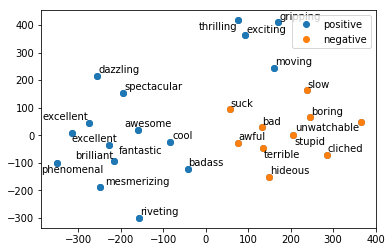
\includegraphics[width=\linewidth,height=\textheight,keepaspectratio]{figs/adjectives.png}
  \caption{T-SNE projection of sentiment indicators}
  \label{fig:adj-fig}
\end{figurehere}


I also employ a technique for visualising word vectors as heatmaps (Li et al. 2015) \cite{viz}. Each column shows the difference from the mean of each component in each word embedding. The influence of a word embedding is determined by its deviation from the mean vector, since these vectors will contribute more to learned document embeddings. From this, we can hypothesise that more importance is placed on key sentiment indicators - e.g. `hate'. In addition, words connecting clauses (e.g. `although') and negating clauses e.g. `not') are salient, since they can change the meanings of parts of the document. An example of this is shown in Figure \ref{fig:var-fig}, in the phrase \textit{``I hate the movie, although the plot is interesting"}, where we can see that the words hate, although, plot and interesting are the most salient. Here, a negative clause is combined with a positive clause, with the overall class being negative - this can be seen on the heatmap, with `hate' being the more salient adjective.

\begin{figure*}
  \centering
  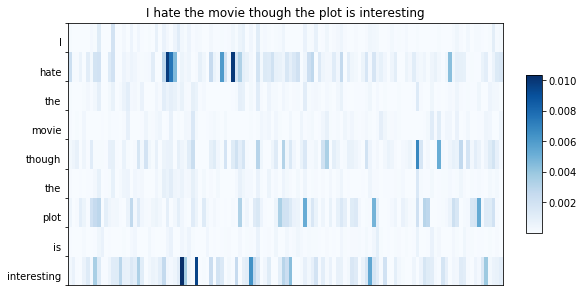
\includegraphics[width=\linewidth,keepaspectratio]{figs/variance_plot.png}
  \caption{Plot of deviation from the mean of word vector components}
  \label{fig:var-fig}
\end{figure*}

\begin{figure*}
  \centering
  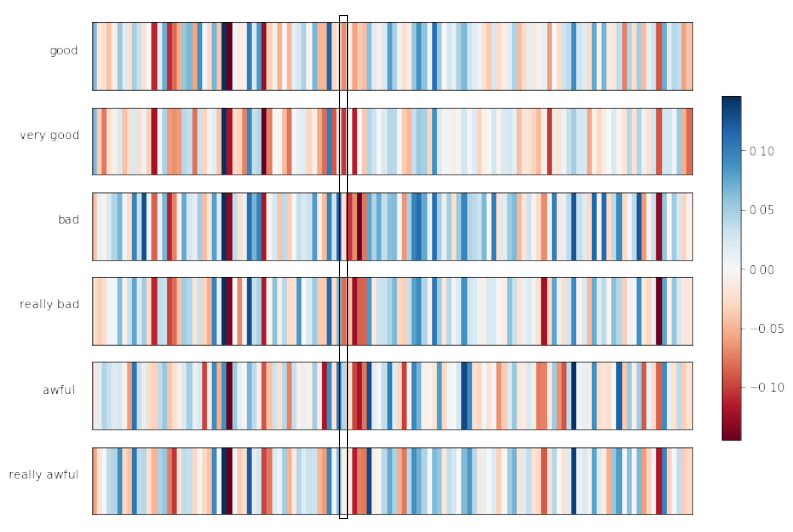
\includegraphics[width=\textwidth,height=\textheight,keepaspectratio]{figs/intense1.png}
  \caption{Plot of document embeddings for phrases and their intensifications}
  \label{fig:intense-fig}
\end{figure*}


\begin{figure*}
  \centering
  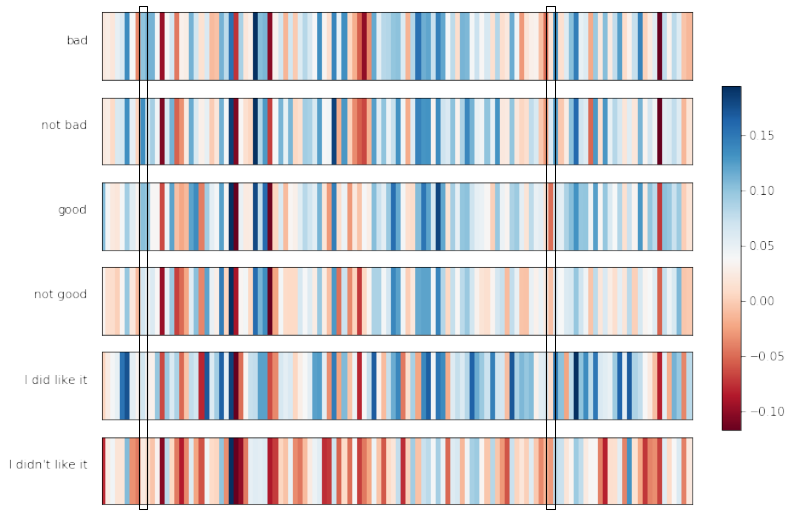
\includegraphics[width=\textwidth,height=\textheight,keepaspectratio]{figs/negate1.png}
  \caption{Plot of document embeddings for phrases and their negations}
  \label{fig:negate-fig}
\end{figure*}


We can also visualise entire document vectors as heatmaps, allowing us to see the effect of intensification and negation. Figures \ref{fig:intense-fig} and \ref{fig:negate-fig} show the document vectors for several short phrases and their modifications. Some patterns can be seen (qualitatively) here, with certain dimensions changing on negation, e.g. the ones highlighted on the figure. With negation, we also observe the difference between entire embeddings for different classifications, since a negated positive document is classified negative. For example, the difference between ``I did like it'' and ``I didn't like it' is clear. The pattern for intensification is more difficult to see, since we expect these modifiers to keep the classification the same, but with higher confidence.



The T-SNE projection in figure \ref{fig:tsne-docs} also shows how negation affects documents embeddings - vectors for phrases and their negations are plotted along with some random common words, to show clustering. This shows negations representing a similar shift in vectors, similarly to word2vec, where analogous pairs (here negation) will have similar vector differences \cite{DBLP:journals/corr/ChenPG17}.


\section{Conclusion}

I have shown that doc2vec produces a representation, that when paired with an SVM model, can outperform a bag-of-words representation. Despite not being directly interpretable, doc2vec still creates a meaningful semantic space for documents, and we can visualise vectors in this space to show this.

\begin{figurehere}
  \centering
  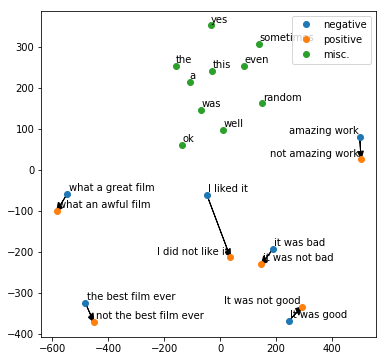
\includegraphics[width=\linewidth,height=\textheight,keepaspectratio]{figs/tsne-docs.png}
  \caption{t-SNE projection of document embeddings of phrases and their negations}
  \label{fig:tsne-docs}
\end{figurehere}
\end{multicols}
\clearpage
\bibliography{refs}




\end{document}
